\documentclass[titlepage]{article}


% Packages
\usepackage[margin=1in]{geometry}
\usepackage{amsmath}
\usepackage{float}
\usepackage{graphicx}
\usepackage[hidelinks]{hyperref}
\usepackage{pdfpages}
\usepackage[nottoc,numbib]{tocbibind}


% Title Info
\title{Pet Caller\\ Prototype 1}
\author
{
    Jade Fjestad\\
    Jesse Lim\\
    Justin Ross\\
    Andreas Smit
}
\date{February 7, 2020}


\begin{document}
    \maketitle

    \section{Product Description}
    \subsection{What our product is?}
    Our product is a device designed to help pet owners manage their
    pets. If a pet owner lets their pets outside they may run into an
    issue of not knowing when their pet wants inside without standing by
    the door waiting for hours. Our product seeks to solve this by
    allowing the pet to ``notify" their owner that they would walk back
    inside. This is done through a transmitter placed on the pets caller
    which sets off an alarm when the pet gets close to the door to be
    let inside. This allows the pet owner to not worry about their
    dog or cat waiting outside their door. No more worrying that your
    dog or cat is cold waiting outside your door.

    \subsection{Use Case}
    This product is designed for those individuals who may not be able
    to hear their animal waiting outside their door to be let in. It is
    often that people have a walkout basement where they don’t realize
    their animal is ready to come in. Or the individual may themselves
    be hard of hearing and cannot hear their quiet cat politely ask to
    come in.

    This product comes in two parts: a hub, and a Caller Fob. The hub
    is a battery powered device that you place on the wall near the door
    your animal comes in. (Sticky tabs included) (same with batteries).
    There is a dial, a power button and a light indicator.
    To set the activation distance (the distance your animal has to be
    to the device to activate the alert), start by placing the Caller
    Fob about where your animal will want to come in, just leave it on
    the ground. Now go to the hub and hold down the power button for 3
    seconds, you will here a sound when you first press down the button
    then another one once you hold it for 3 seconds. To increase the
    activation distance begin to turn the adjustment dial clockwise
    until you hear a continuous sound, the sound indicates the Caller
    Fob is now in the calling range of the hub.
    To confirm this distance press the power button once more and the
    device will use this distance and turn off. Now attach the Caller
    Fob to your pets collar.
    To adjust the volume just turn the dial, while the device is active.
    To activate the device turn on the power button, the led should turn
    on. The hub will now alert you when the Caller Fob is in the
    activation range of the device and your pet has been waiting there
    for 15 seconds. The sound notification will notify the user the pet
    wants to come in. To deactivate the device when your
    pet returns, press the power button once again. (and the LED will
    turn off). We suggest you only turn on the device when you let your
    animal out and then turn it off when your animal comes inside, to
    help prevent accidental activation of the alert.


    \subsection{Advantages to Similar Products}
    This item is superior to the cat/dog door because there are issues
    with this method of solving the problem. Conventional Cat/Dog doors
    allow all animals not only your pets into your house and in colder
    climates, these small openings cause your house’s heating to easily
    escape. With this product you have more control over your animals
    coming and going.

    \subsection{User Persona}
    \subsubsection{User life improvements from product}
    This product will improve the quality of life of your pet. It will
    allow you to have more freedom in your house when your animal is
    outside in the cold of winter or late at night.
    You don’t have to worry about other rodents entering your house
    through a cat or doggy door, since now you have full control over
    your pets comings and goings.
    \subsubsection{Potential Users}
    According to the American Veterinary Medical Association 38.4\% of
    Americans own a dog and 25.4\% of Americans have a cat
    \cite{pet_owner}. This gives us a large number of potential users in
    the area of North America.
    \subsubsection{Possible downsides of Product}
    This product will improve the quality of life of your pet. It will
    allow you to have more freedom in your house when your animal is
    outside in the cold of winter or late at night.
    You don’t have to worry about other rodents entering your house
    through a cat or doggy door, since now you have full control over
    your pets comings and goings.
    \subsubsection{Persona}
    Name: Sabastian Müller
    He is a stay at home dad with girls of ages 5 and 3. They have a
    large house with a walkout basement. They have a playroom on the
    main floor and a young dog, Salt, that enjoys playing with the
    neighbor's dog since their yards are connected. They trained their
    dog to not bark, so she is more well behaved, but this causes an
    issue when to let the dog in.
    He worries that his girls may get into mischief if he were to spend
    too much time away from them. He hopes that he can get work done
    while he watches his girls and his dog is outside.
    He hears on an targeted ad that there is this device that can help
    him remain upstairs while his dog is outside. He thinks, “Oh this
    would be great! So I can watch the girls and let my dog out when it
    gets cold and not have to worry about Salt getting too cold. I
    should buy this right away.”.
    He values a product that will allow him to rest his mind while his
    dog is outside.



    \pagebreak
    \section{Technical Details}
    \subsection{BOM and cost projection}
    Table \ref{tab:BOM} shows a rough estimate of our prices for the
    product.
    \begin{table}[H]
        \caption{Bill of Materials}
        \label{tab:BOM}
        \centering
        \begin{tabular}{c|c}
            \textbf{Item} & \textbf{Cost} \\
            \hline
            PIC 32 processor & $\$ 10.00$ \\
            Cortex M3 Razor Board & $\$ 90.00$ \\
            Audio Equipment & $\$ 30.00$\\
            ANT transmitter & $\$ 20.00$\\
            Batteries & $\$ 5.00$\\
            Casing & $\$ 10.00$\\
            Misc Electronics & $\$ 10.00$\\
            \hline
            \textbf{Total} & $\$ 175.00$\\
        \end{tabular}
    \end{table}%
    Clearly this is an estimate of prices for a prototype. In the final
    product a custom built board could be made for both the hub and tag
    that would reduce the price as opposed to buying pre-build boards
    with extra functionality. For example the only need for the Cortex
    M3 board is for a processor on it costing a total of $\$ 4.00$. It
    would probably be feasable to keep the total cost of production to
    under $\$ 100$, giving an estimated unit cost of potentially
    somewhere from $\$ 150.00$ to $\$ 200.00$.

    \subsection{Mechanical Design}
    See the mechanical design documents attached in appendix
    \ref{sec:mec_draw} for the specifications of the mechanical design.

    \subsection{Electrical Design}
    The majority of the operation of the product is done through the PIC
    32 processor. The use of the external processors is simply for the
    communication via the ANT wireless protocol. A rough block schematic
    is shown in appendix \ref{sec:elec_draw}.

    \subsubsection{Wireless Communications}
    The ANT wireless protocol was chosen for the wireless communication
    between the collar tag and the base station. The wireless base
    station will most likely be driven by the Cortex M3 board if
    approved. The transmitter will most likely be driven through the use
    of a SparkFun NRF52832 breakout board (SparkFun product number
    \href{https://www.sparkfun.com/products/13990}{13990}).
    The ANT wireless protocol is chosen for multiple reasons. The
    largest one is three of our group members are currently learning
    ANT through the Embedded in Embedded program offered by Jason Long.
    Secondly ANT has multiple advantages as a low energy wireless
    protocol given from the ANT website \cite{ant_site} including,
    \begin{itemize}
        \item Ultra Low power, can be run on a coin cell for years
        \item Easy to use - The protocol specification is only 100 pages
            long
        \item Low Cost
    \end{itemize}
    For these reasons especially the ease of use and cost we will use
    ANT. Should ANT not be possible RFID or some sort of physical
    interaction could be used to trigger the device.

    \appendix

    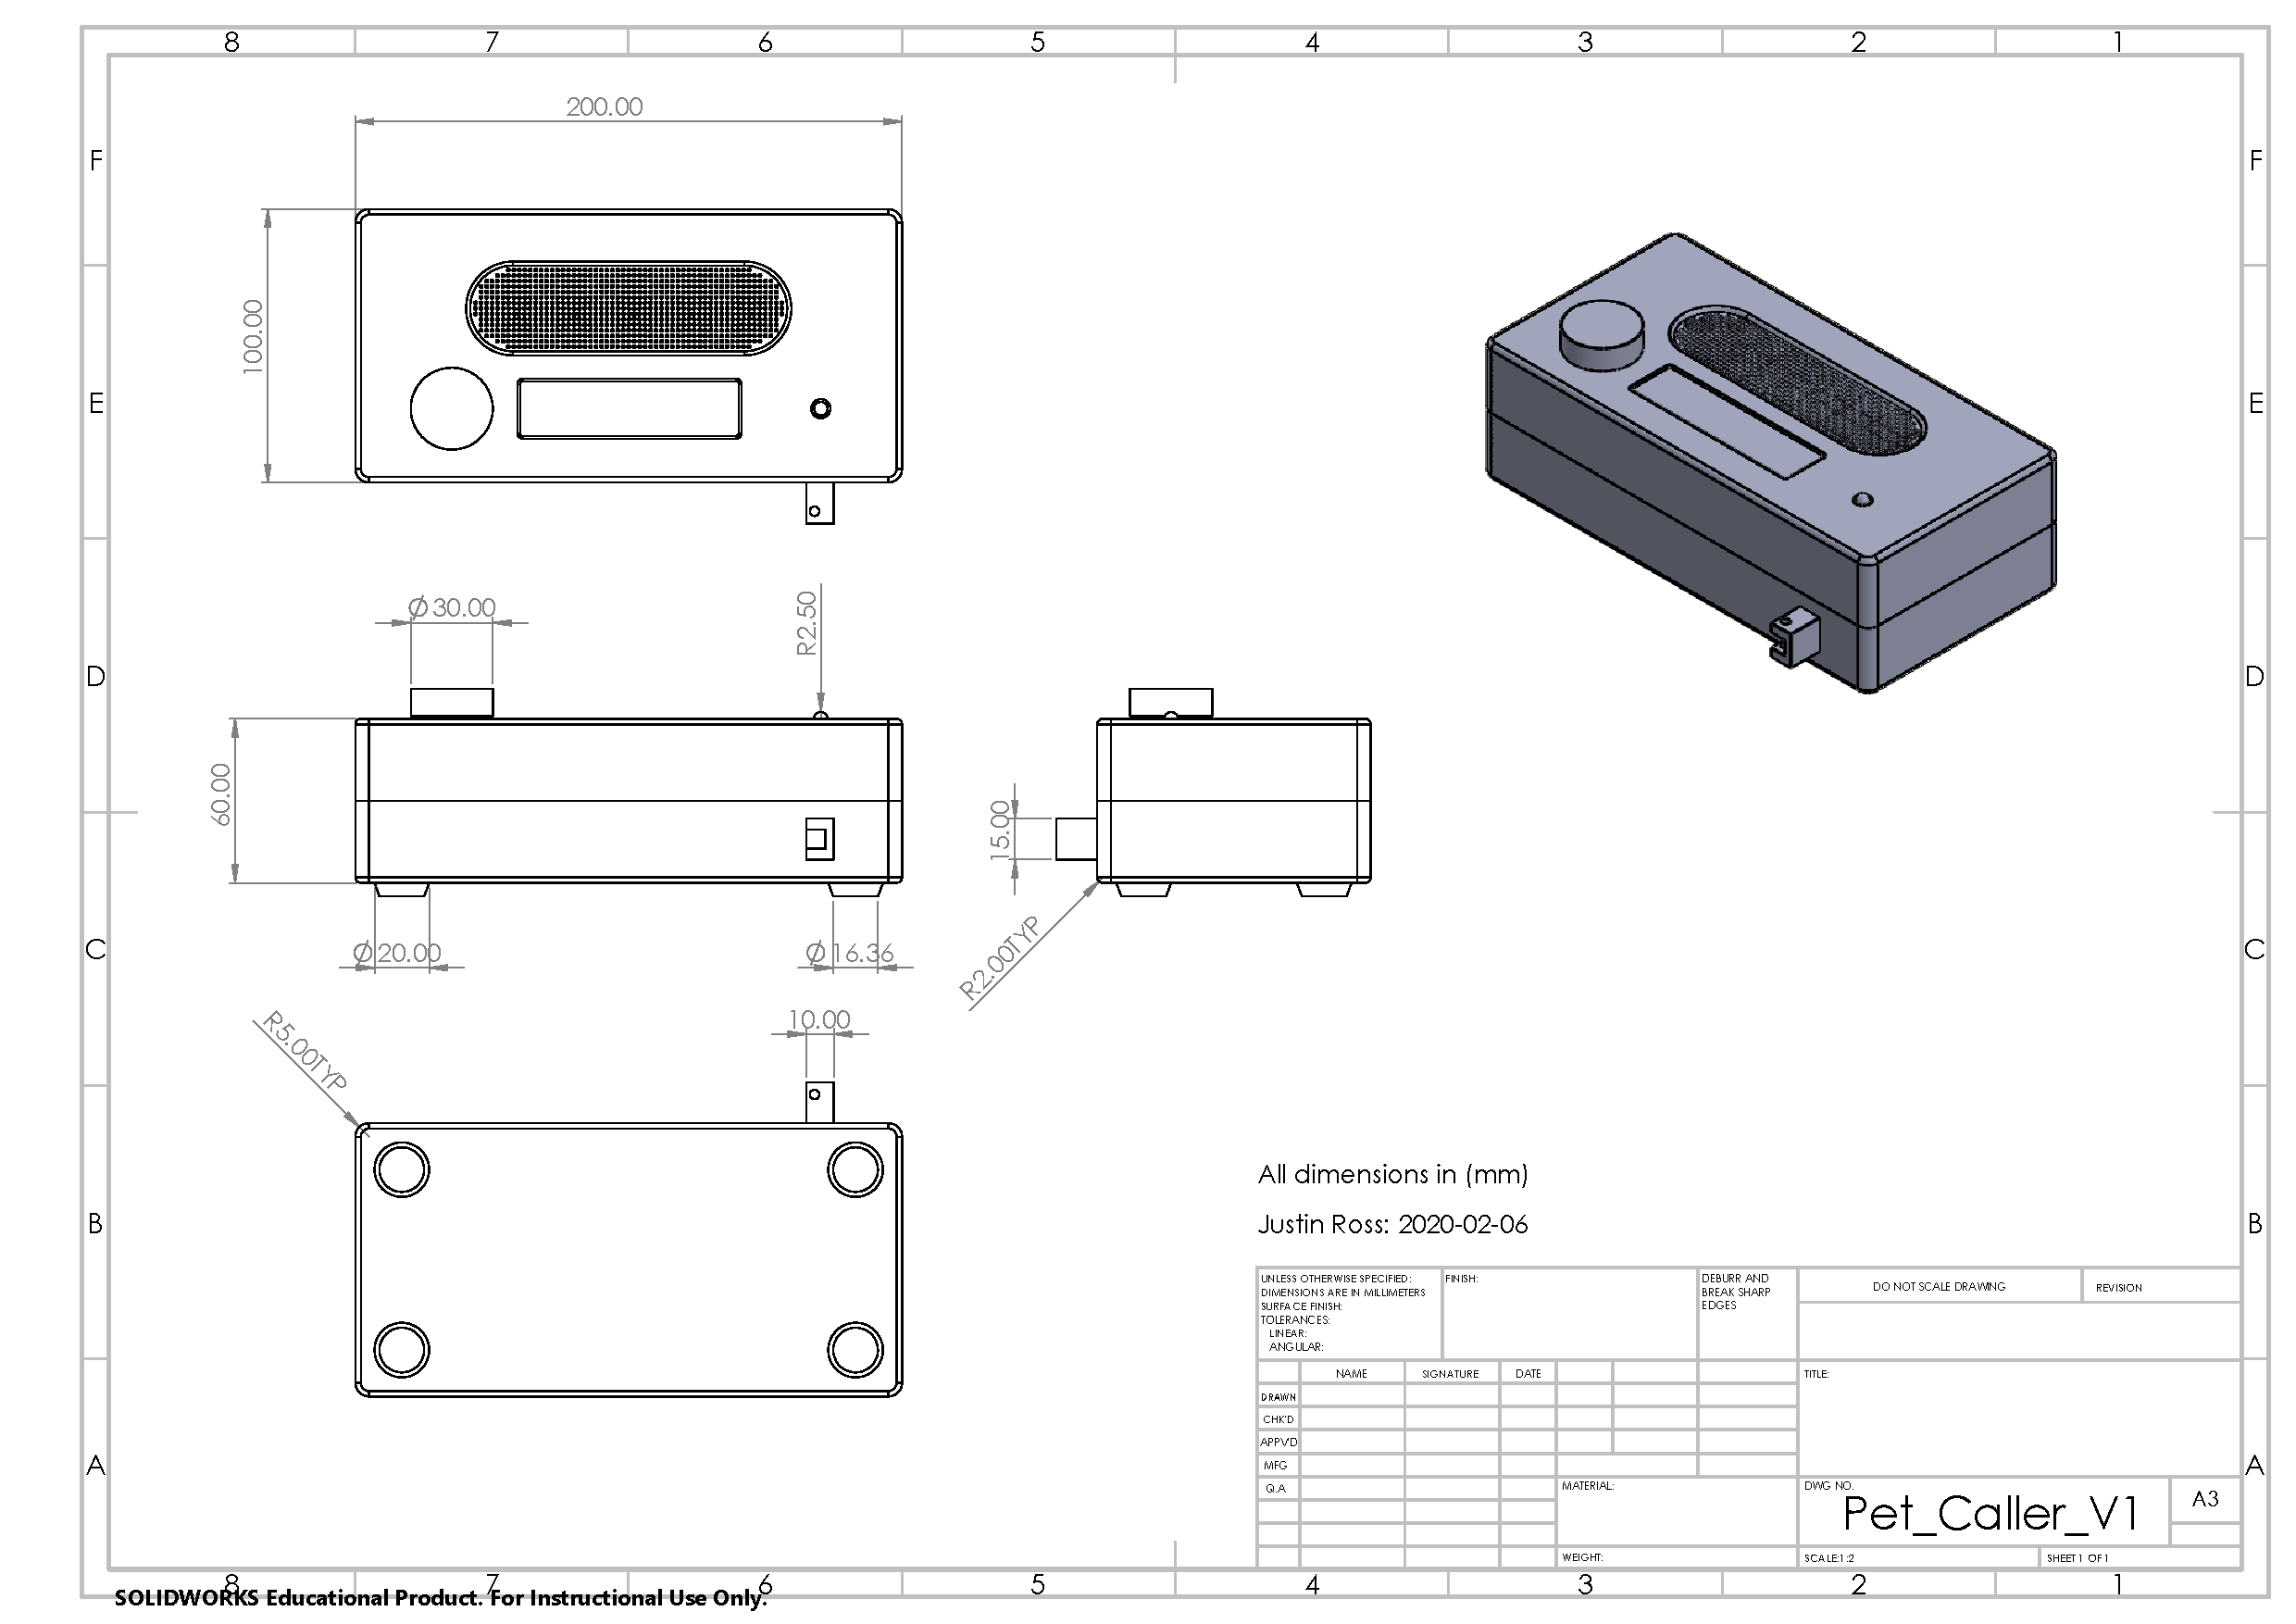
\includepdf[scale=0.9, offset=0mm -75, pagecommand=
    {
        \section*{Appendices}
        \section{Mechanical Design Drawings}\label{sec:mec_draw}
    }]{Pet_Caller_V1.pdf}
    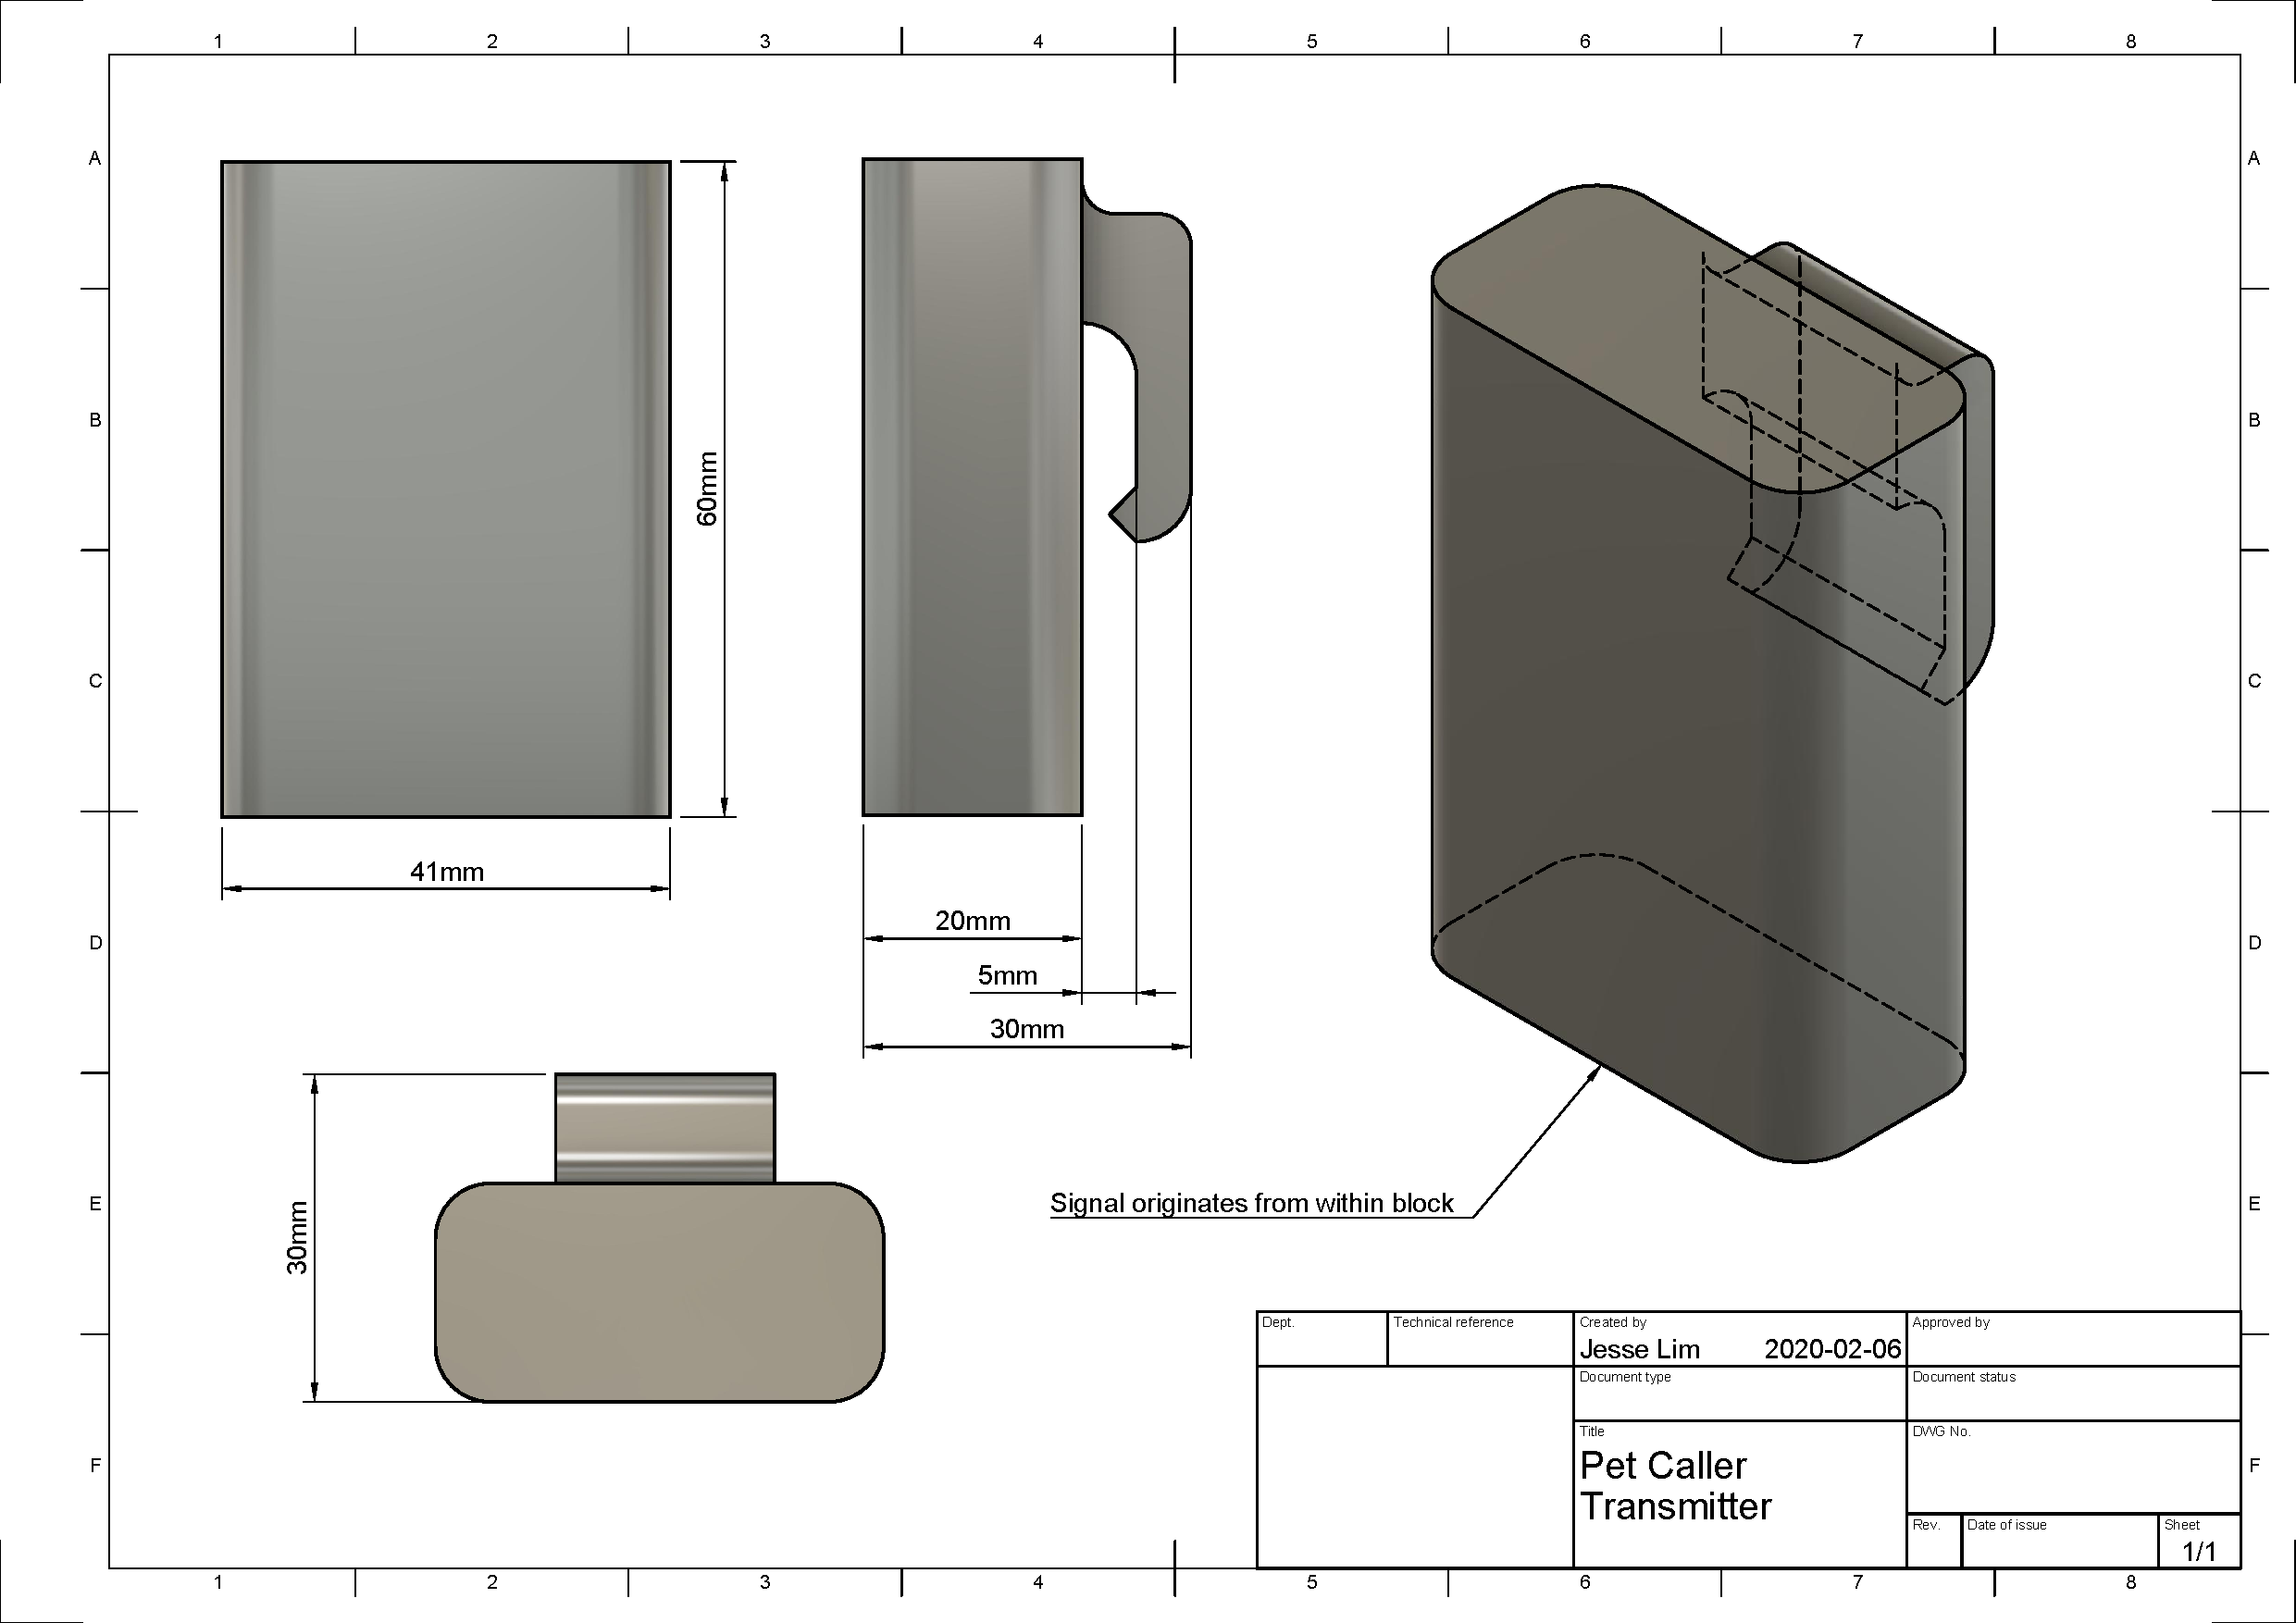
\includepdf[scale=0.9]{Transmitter_v1.pdf}

    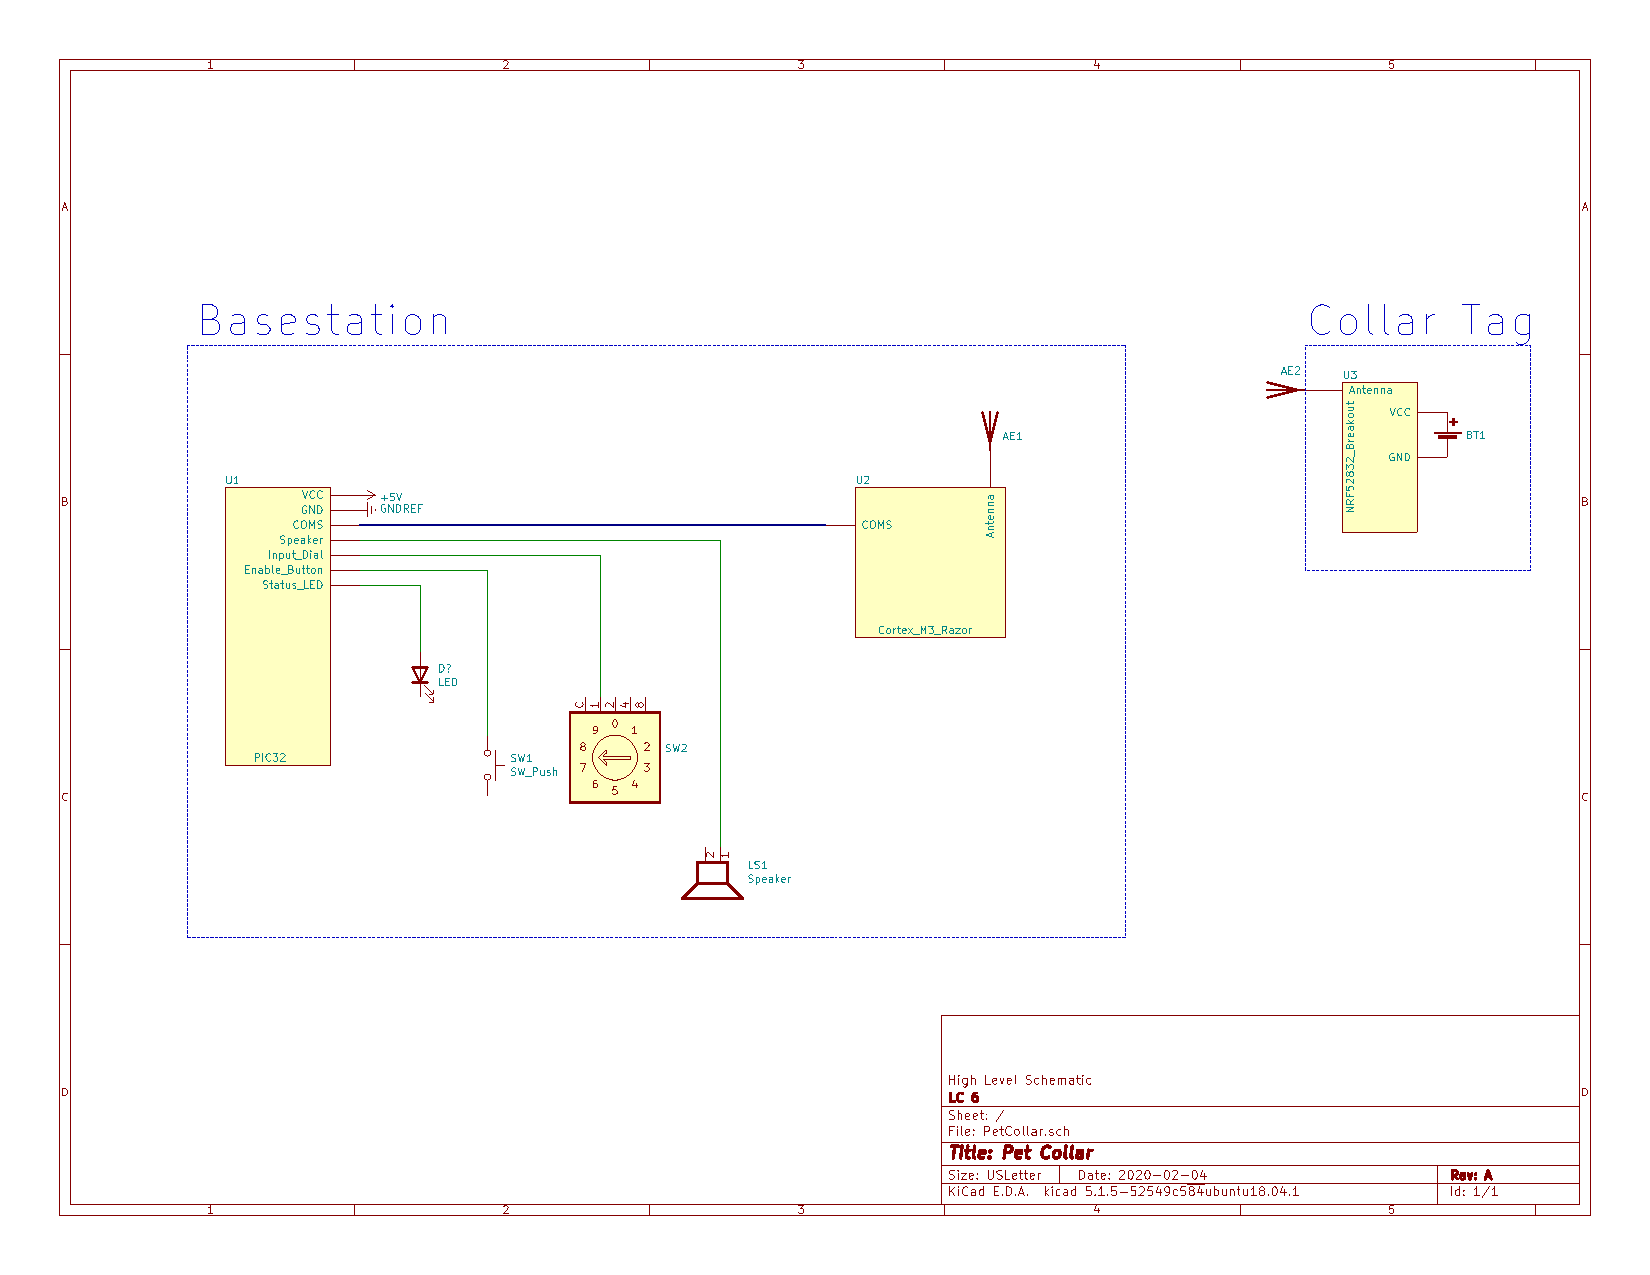
\includepdf[scale=0.9, offset=0mm -75, pagecommand=
    {
        \section{Electrical Design Drawings}\label{sec:elec_draw}
    }]{PetCollar.pdf}

    \bibliographystyle{IEEEtran}
    \bibliography{ref}
\end{document}
